\begin{questions}
	\question Paralléliser le code séquentiel initial avec OpenMP.
	\begin{solution}
		Avant de foncer tête baissée, il est bon de refléchir un peu et de trouver où l'on passe le plus de temps : c'est cette zone qu'il faut essayer de paralléliser.
		Ici, il n'est pas question d'utiliser des primitives très complexes, un simple \texttt{\#pragma omp parallel for schedule(runtime)} devrait suffir.
		Vous pourrez ensuite définir, à l'exécution du code, les variables d'environnement \texttt{OMP\_NUM\_THREADS} et \texttt{OMP\_SCHEDULE} afin de trouver le meilleur compromis pour les performances. 
	\end{solution}

	\question Créer une structure MPI (\texttt{bodyMPI}) pour envoyer/recevoir des corps.
	\begin{solution}
		La structure \texttt{body} qui est déclarée dans le fichier \textit{src/body.h} ne fait pas partie des types de base que connaît MPI.
		Il faut donc déclarer une nouvelle structure MPI suivant les spécifications de la structure \texttt{body}.
		La création de structure MPI est assurée par la routine \texttt{MPI\_Type\_struct}.
		Une fois la structure MPI créée il faut nécessairement la déclarer avec la routine \texttt{MPI\_Type\_commit}.
		Avant de quitter le programme il faut penser à libérer la mémoire utilisée par la structure en appelant \texttt{MPI\_Type\_free}.
		Vous pouvez vous référer au code proposé dans \textit{src/help/stuctureMPI.c} si vous le souhaitez.
	\end{solution}

	\question Mettre en place un anneau de communication MPI (voir fig.~\ref{fig:anneau}).
	\begin{figure}[htbp]
		\centering
		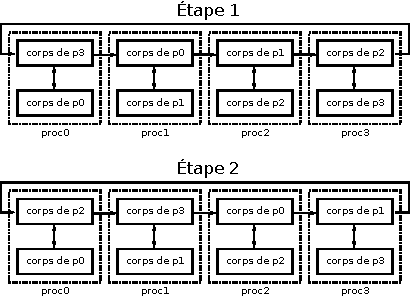
\includegraphics[width=0.6\linewidth]{schemas/anneau_sans_buffering.pdf}
		\caption{Anneau de communication pour 4 processus MPI}
		\label{fig:anneau}
	\end{figure}
	\begin{solution}
		Une itération est complète quand tous les processus MPI ont reçu les corps de tous les autres processus.
		Pour y parvenir il y a deux phases:
		\begin{itemize}
			\item le calcul des accélérations des corps locaux entre eux (au sein d'un même processus),
			\item le calcul des accélérations des corps locaux en fonction des corps des autres processus.
		\end{itemize}
		Si il y a $np$ processus MPI, alors il y a $np-1$ communications.
		Dans un premier temps, il faudra déterminer le rang des processus précédent et suivant dans l'anneau pour chaque n\oe ud MPI.
		%Ensuite, on utilisera un unique \texttt{buffer} pour envoyer et recevoir les corps.
		%Avant chaque envoie de corps il faudra bien penser à copier les corps locaux dans le \textit{buffer} MPI.
		%Comme il est impossible d'envoyer et de recevoir en même temps (\textit{buffer} MPI unique), il faudra déterminer qui envoie et qui reçoit en fonction du rang MPI.
		%La réception et l'envoi peuvent être réalisés de façon bloquante avec les routines \texttt{MPI\_Recv} et \texttt{MPI\_Send}.
		Se référer à la question suivante pour plus de précision sur l'implémentation.
	\end{solution}

	\question Implémenter le \textit{double buffering} (cf. fig.~\ref{fig:anneauDB}).
	\begin{figure}[htbp]
		\centering
		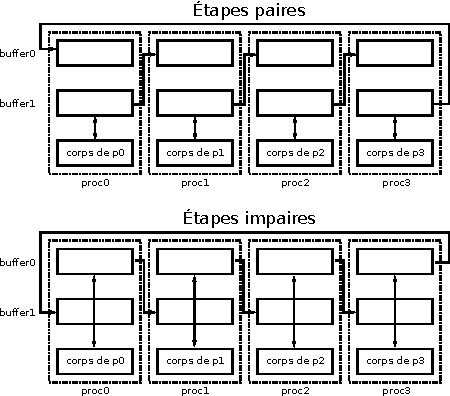
\includegraphics[width=0.65\linewidth]{schemas/anneau_avec_buffering.pdf}
		\caption{Anneau de communication pour 4 processus MPI avec \textit{double buffering}}
		\label{fig:anneauDB}
	\end{figure}
	\begin{solution}
		Chaque processus possèdera deux \textit{buffers} MPI: un pour l'envoi et l'autre pour la réception.
		À chaque étape d'une itération il faudra bien penser à intervertir ces deux \textit{buffers}: le \textit{buffer} d'envoi deviendra le \textit{buffer} de réception et vice versa.
		Cette implémentation permet:
		\begin{itemize}
			\item d'envoyer et de recevoir des corps en même temps,
			\item d'envoyer et de recevoir des corps pendant que l'on calcule l'accélération avec d'autres corps.
		\end{itemize}
		Dans un premier temps vous implémenterez le \textit{double buffering} avec les communications MPI bloquantes (voir les routines \texttt{MPI\_Recv} et \texttt{MPI\_Send}).
		%Le \textit{double buffering} permet d'éviter ce problème en utilisant deux \textit{buffers} MPI au lieu d'un seul.
		%Il est ainsi possible d'envoyer des corps à un processus même si ce dernier n'a pas terminé ses traitements.
		%Attention, il faudra bien penser à inverser les \textit{buffers} à chaque étape (au sein d'une même itération) pour que cela fonctionne: un coup on reçoit dans le \texttt{buffer0} et le coup d'après on reçoit dans le \texttt{buffer1}.
		%Cette implémentation devrait déjà grandement améliorer les performances en supprimant des recopies de mémoire inutiles.
		%Cependant le recouvrement calcul-communication n'est toujours pas possible à cause des communications bloquantes (\texttt{MPI\_Recv} et \texttt{MPI\_Send}).
		%L'exercice suivant permet de lever cette limitation.
	\end{solution}

	\question Trouver le plus petit pas de temps $dt$ parmi tout les processus MPI et le choisir.
	\begin{solution}
		À chaque itération, un nouveau pas de temps est calculé en fonction de la position des corps dans le plan.
		Dans la version parallèle à mémoire distrubuée il est impératif que tous les processus MPI aient le même $dt$.
		Pour y parvenir il faut utiliser une réduction de type minimum (voir \texttt{MPI\_Allreduce}).
		Il doit maintenant être possible de lancer la simulation sur plusieurs n\oe uds.
	\end{solution}
\end{questions}

\section{Bonus}
Si vous êtes arrivé ici c'est surement parce que vous êtes à l'aise et à partir de maintenant, le sujet sera volontairement moins précis.
Si jamais vous rencontrez des difficultés n'hésitez pas à demander.
L'objectif de cette partie est de traiter le recouvrement des communications par du calcul.
Ce recouvrement est théoriquement possible dans le cas du prolème à $N$ corps car il y a $O(N^2)$ calculs pour $N$ données à échanger.\\

\begin{questions}
	\question Utiliser les communications MPI non bloquantes.
	\begin{solution}
		Les communications non bloquantes permettent d'envoyer et de recevoir des \textit{buffers} pendant que l'on calcule.
		Voir les routines \texttt{MPI\_Isend}, \texttt{MPI\_Irecv} et \texttt{MPI\_Wait}.
	\end{solution}

	\question Utiliser les communications MPI persistantes.
	\begin{solution}
		Les communications persitantes permettent de factoriser les temps d'initialisation des communications MPI.
		Soit $t_1$ le temps d'initialisation de l'envoi d'un \textit{buffer}, $t_2$ le temps de l'envoi du \textit{buffer} et $t_3$ le temps d'initialisation de la réception:
		\begin{equation*}
			t_{com} \simeq t_1 + t_2 + t_3
		\end{equation*}
		Les communications persistantes permettent de diminuer fortement $t_1$ et $t_3$.
		Voir les routines \texttt{MPI\_Send\_init}, \texttt{MPI\_Recv\_init}, \texttt{MPI\_Start} et \texttt{MPI\_Wait}.
	\end{solution}

	\question Utiliser les communications MPI persistantes collectives.
	\begin{solution}
		Cela ne change pas grand chose en terme de performance mais permet de factoriser du code en fusionnant l'appel à l'envoi et à la réception des \textit{buffers}.
		Voir les routines \texttt{MPI\_Startall} et \texttt{MPI\_Waitall}.
	\end{solution}
\end{questions}
